\section{Testing}
These properties are all expected to hold within 2PL. This should be true with respect to both Strict 2PL and Conservative 2PL. However, their implication to serializability rests on order assumptions. DBCheck does not have a serializable order defined for all models. For the naive model and strict 2PL there is no order defined for the model. In C1 and C2PL, the models do have an order defined.  The final property is the deadlock property. This is defined loosely as 
AF ( p1.finished \& p2.finished)
The meaning of this is that in all states there exists a future state where both processes have finished.


\begin{tabular}{l||llll}
&Deadlock&WW&WR&RW\\\hline
Simple 2op&64/256&216/256&216/256&144/256\\
S2PL 2op&256/256&256/256&256/256&256/250\\
C2PL 2op&256/256&256/256&256/256&256/250\\
Naive 4op&<++>/65536&<++>/65536&<++>/65536&<++>/65536\\
S2PL 4op&<++>/65536&<++>/65536&<++>/65536&<++>/65536\\
C2PL 4op&65536/65536&65536/65536&65536/65536&65536/65536\\
\end{tabular}


From the results above, the stated behavior of strict 2pl and c2pl can be observed. Strict 2pl succeeds on all the serialzability specifications but does not on the deadlock specification. Conservative 2pl succeeds on all specifications. As expected a simple lock does not meet the serializability criterion. 

\section{Samples}
\subsection{S2PL Deadlock}
Shown below is an example of the S2PL lock in deadlock. This example is pulled from a counterexample generated in testing the deadlock specification on a S2PL configuration.

\begin{figure}[H]
	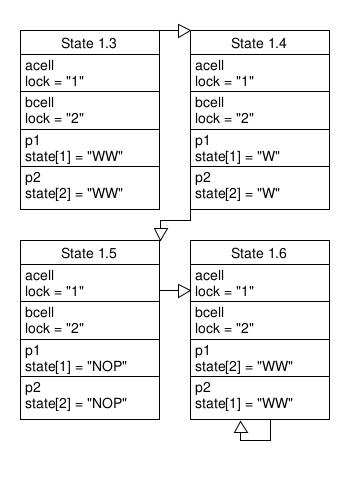
\includegraphics[width=\linewidth]{2pl_deadlock.jpg}
\end{figure}

\subsection{Simple Lock WW Failure}
This figure shows the state diagram of a counterexample for the WW serializability spec. The simple lock is not designed for schedule serializability. The figure shows an example of the specification not holding for the model.

\begin{figure}[H]
	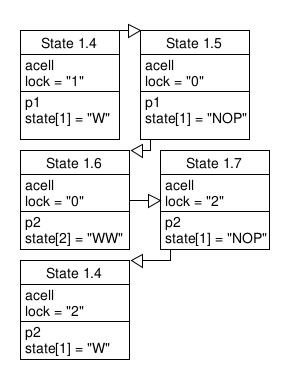
\includegraphics[width=\linewidth]{simple_WW.jpg}
\end{figure}
